% fig_hier -- containment, in the visual language of fig_ops: a WIDE strip, blue for sets, green
% for fields, red for operators, a bold name + its symbol underneath. Read left to right = coarser.
%
% Three levels only: molecules, cells, tissues. The organism panel held one box of anonymous dots
% and no set of its own, so it showed the containment map repeating rather than anything new.
%
% THE POINT THE FIGURE HAS TO MAKE is that a parent holds SEVERAL DISTINCT SETS, not one kind of
% child: the cell at S1 contains receptors, signalling proteins and cytoskeleton, drawn as three
% different marks, each its own set with its own state. Red arrows are operators -- within a level
% (receptor -> signalling -> cytoskeleton) and across it (Aggregate up, Broadcast down). Green is a
% field, bound to one level and reached by Exchange.
\documentclass[border=5pt]{standalone}
\usepackage{amsmath,amssymb}
\usepackage{xcolor}
\usepackage{tikz}
\usetikzlibrary{positioning,arrows.meta,fit,backgrounds,calc,shapes.geometric}
\definecolor{cset}{RGB}{31,119,180}
\definecolor{cfield}{RGB}{44,160,44}
\definecolor{cop}{RGB}{214,39,40}
\definecolor{cgray}{RGB}{120,120,120}
\begin{document}
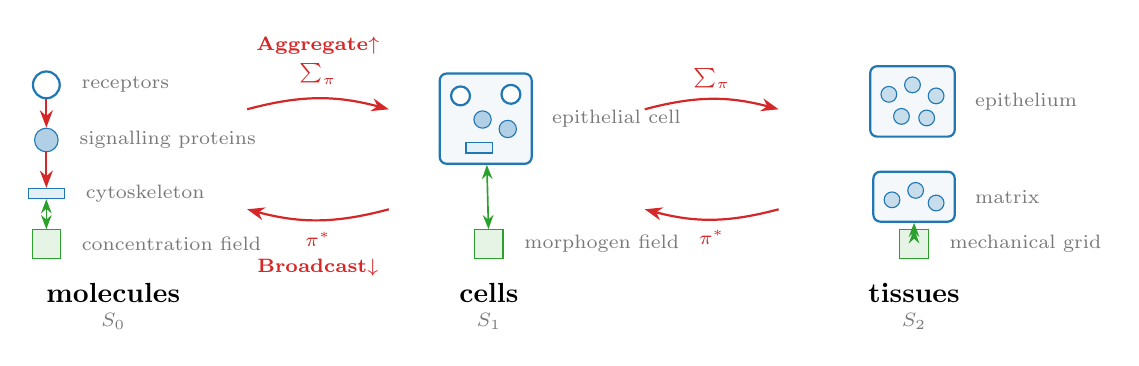
\begin{tikzpicture}[
  font=\footnotesize,
  % one MARK per set, so "distinct set" is visible at a glance and survives being shrunk
  recept/.style={circle,draw=cset,thick,fill=white,minimum size=3.4mm,inner sep=0pt},
  sig/.style={circle,draw=cset,fill=cset!35,minimum size=3.0mm,inner sep=0pt},
  cyto/.style={draw=cset,fill=cset!12,minimum width=4.6mm,minimum height=1.3mm,inner sep=0pt},
  tiny/.style={circle,draw=cset,fill=cset!25,minimum size=2.0mm,inner sep=0pt},
  cellbox/.style={draw=cset,thick,rounded corners=2.5pt,fill=cset!5,inner sep=1.3mm},
  lab/.style={font=\scriptsize,color=cgray},
  ttl/.style={font=\bfseries},
  fld/.style={draw=cfield,fill=cfield!12,minimum size=3.6mm,inner sep=0pt},
  op/.style={-{Stealth[length=2.2mm]},cop,thick},
  ex/.style={{Stealth[length=1.8mm]}-{Stealth[length=1.8mm]},cfield,semithick},
]

% =========== S0: three distinct sets, and operators BETWEEN them ============
\node[recept] (r0) at (0,0.86) {};
\node[sig]    (s0) at (0,0.16) {};
\node[cyto]   (k0) at (0,-0.52) {};
\node[lab,right=1.4mm of r0] {receptors};
\node[lab,right=1.4mm of s0] {signalling proteins};
\node[lab,right=1.4mm of k0] {cytoskeleton};
\draw[op] (r0) -- (s0);
\draw[op] (s0) -- (k0);
\node[fld] (fld0) at (0,-1.16) {};
\node[lab,right=1.4mm of fld0] {concentration field};
\draw[ex] (fld0) -- (k0);
\node[ttl] at (0.85,-1.78) {molecules};
\node[lab] at (0.85,-2.14) {$S_0$};

% =========== S1: ONE cell holding all three of those sets ==================
\begin{scope}[shift={(5.6,0)}]
  \node[recept,minimum size=2.4mm] (r1) at (-0.34,0.72) {};
  \node[recept,minimum size=2.4mm] (r1b) at ( 0.30,0.74) {};
  \node[sig,minimum size=2.2mm]    (s1) at (-0.06,0.42) {};
  \node[sig,minimum size=2.2mm]    (s1b) at ( 0.26,0.30) {};
  \node[cyto,minimum width=3.4mm]  (k1) at (-0.10,0.06) {};
  \begin{scope}[on background layer]
    \node[cellbox,fit=(r1)(r1b)(s1)(s1b)(k1)] (cellA) {};
  \end{scope}
  \node[lab,right=1.2mm of cellA] {epithelial cell};
  % THE NEURON BOX IS GONE. It sat at y=-0.55 as a second cell-level set, and the Exchange arrow
  % reached the morphogen field through it. The point S1 has to make -- one parent holding SEVERAL
  % DISTINCT SETS -- is already made by `cellA`, which holds receptors, signalling proteins and
  % cytoskeleton; S2's epithelium + matrix makes the sibling-sets point at the next level up. The
  % neuron made neither point twice over and cost the panel a mark the caption never named. The
  % Exchange now binds the field to the cell it actually couples to.
  \node[fld] (fld1) at (0.02,-1.16) {};
  \node[lab,right=1.4mm of fld1] {morphogen field};
  \draw[ex] (fld1) -- (cellA);
  \node[ttl] at (0.02,-1.78) {cells};
  \node[lab] at (0.02,-2.14) {$S_1$};
\end{scope}

% =========== S2: tissues, each holding cells ===============================
\begin{scope}[shift={(11.0,0)}]
  \node[tiny] (t1a) at (-0.30,0.74) {};
  \node[tiny] (t1b) at ( 0.00,0.86) {};
  \node[tiny] (t1c) at ( 0.30,0.72) {};
  \node[tiny] (t1d) at (-0.14,0.46) {};
  \node[tiny] (t1e) at ( 0.18,0.44) {};
  \begin{scope}[on background layer]
    \node[cellbox,fit=(t1a)(t1b)(t1c)(t1d)(t1e)] (tisA) {};
  \end{scope}
  \node[lab,right=1.2mm of tisA] {epithelium};
  \node[tiny] (t2a) at (-0.26,-0.60) {};
  \node[tiny] (t2b) at ( 0.04,-0.48) {};
  \node[tiny] (t2c) at ( 0.30,-0.64) {};
  \begin{scope}[on background layer]
    \node[cellbox,fit=(t2a)(t2b)(t2c)] (tisB) {};
  \end{scope}
  \node[lab,right=1.2mm of tisB] {matrix};
  \node[fld] (fld2) at (0.02,-1.16) {};
  \node[lab,right=1.4mm of fld2] {mechanical grid};
  \draw[ex] (fld2) -- (tisB);
  \node[ttl] at (0.02,-1.78) {tissues};
  \node[lab] at (0.02,-2.14) {$S_2$};
\end{scope}

% =========== the two operators that cross a level ==========================
\draw[op] (2.55,0.55) to[bend left=15] (4.35,0.55);
\draw[op] (4.35,-0.72) to[bend left=15] (2.55,-0.72);
\node[font=\bfseries\scriptsize,color=cop] at (3.45,1.36) {Aggregate$\uparrow$};
\node[font=\scriptsize,color=cop]          at (3.45,1.00) {$\textstyle\sum_{\pi}$};
\node[font=\bfseries\scriptsize,color=cop] at (3.45,-1.46) {Broadcast$\downarrow$};
\node[font=\scriptsize,color=cop]          at (3.45,-1.10) {$\pi^{*}$};
\foreach \x in {8.45}{
  \draw[op] (\x-0.85,0.55) to[bend left=15]
        node[above,font=\scriptsize,color=cop]{$\textstyle\sum_{\pi}$} (\x+0.85,0.55);
  \draw[op] (\x+0.85,-0.72) to[bend left=15]
        node[below,font=\scriptsize,color=cop]{$\pi^{*}$} (\x-0.85,-0.72);
}

\end{tikzpicture}
\end{document}
